\documentclass{beamer}
\usetheme{Boadilla}
\usepackage{essay-def}
\usepackage{bm}
\usepackage{amsfonts}
\usepackage{amssymb}
\usepackage{amsmath}
\usepackage{amsthm}
\usepackage{comment}
\usepackage{geometry}
\geometry{left=1cm,right=1cm}
    \title[NLG]{Natural language generation as dynamical systems}
\author[J. Zhao]{Jiaxi Zhao}
\date{13th May, 2024}
\begin{document}
\par \setlength{\parindent}{2em}

\begin{frame}
\titlepage

\end{frame}

\begin{frame}[Word embedding: an old story]
	
\end{frame}

\begin{frame}[]
	\begin{figure}
		\centering
		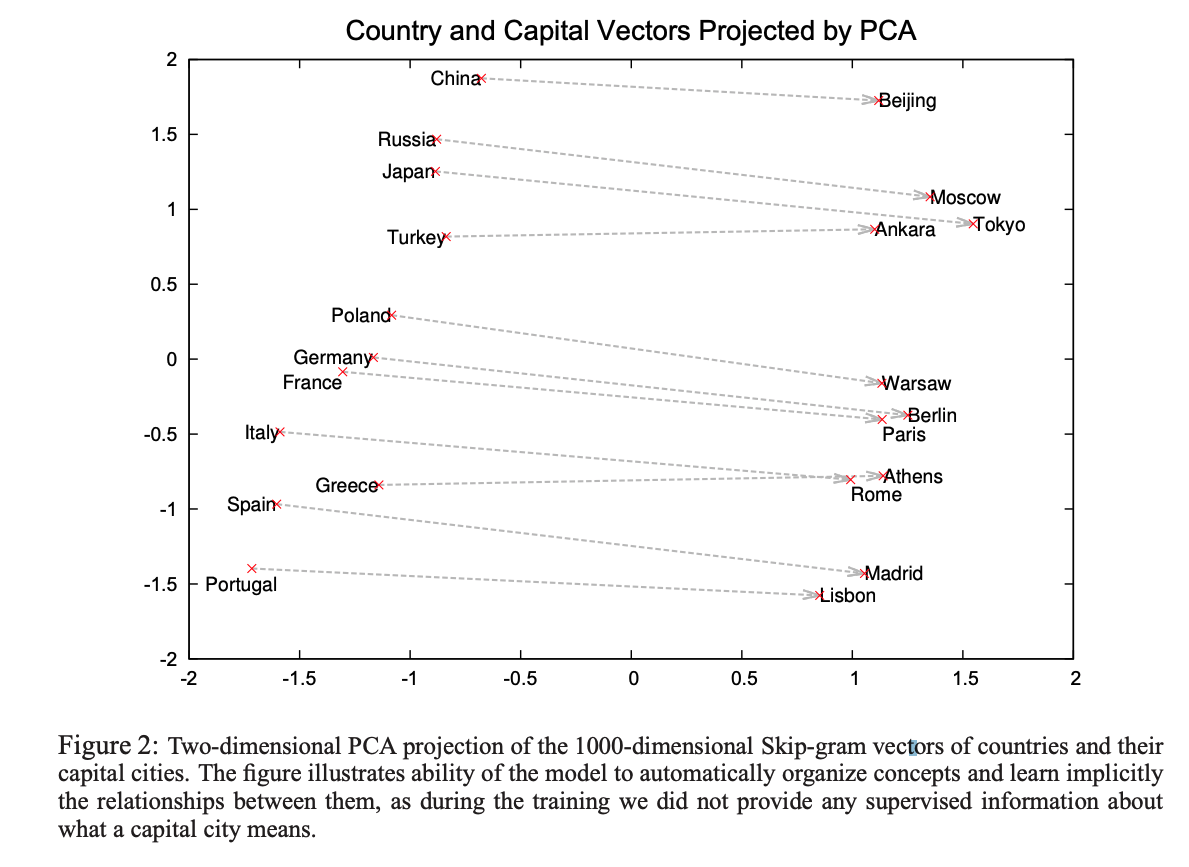
\includegraphics[width=0.8\textwidth]{fig/word2vec.png}
		\caption{Word2Vec}
	\end{figure}
\end{frame}

\begin{frame}[Decoding strategies]
	\begin{itemize}
		\item Greedy decoding
		\item Beam search
		\item Sampling
		\item Top-k sampling
		\item Top-p sampling
	\end{itemize}
	\begin{figure}
		\centering
		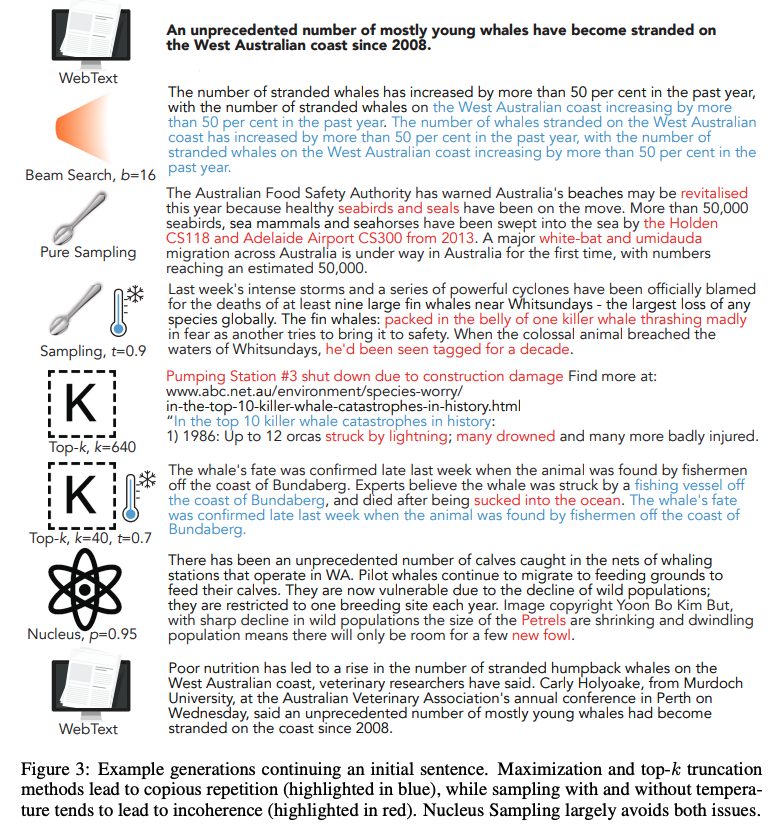
\includegraphics[width=0.8\textwidth]{fig/decoding.png}
		\caption{Word2Vec}
	\end{figure}
\end{frame}

\begin{frame}{Reference}
	\begin{itemize}
		\item 1. Luo, Calvin. "Understanding diffusion models: A unified perspective." arXiv preprint arXiv:2208.11970 (2022).
		\item 2. Ho, Jonathan, Ajay Jain, and Pieter Abbeel. "Denoising diffusion probabilistic models." Advances in Neural Information Processing Systems 33 (2020): 6840-6851.
		\item 3. Tutorial on Denoising Diffusion-based Generative Modeling: Foundations and Applications: https://www.youtube.com/watch?v=cS6JQpEY9cs\&t=1948s
		\item 4. Berkeley CS 285 Lecture 18 note: https://zhuanlan.zhihu.com/p/402237111
	\end{itemize}

\end{frame}







\end{document}